\chapter{NumPy e Matplotlib}\label{numpy}

A lista (\inlcode{list}) em Python é uma estrutura de dados altamente versátil: cada elemento pode conter qualquer tipo
de objeto, independentemente do tamanho ou tipo, e a estrutura pode ser modificada e redimensionada dinamicamente.
No entanto, toda essa generalidade e flexibilidade tem um custo --- especialmente em termos de desempenho.

Diferente de outras linguagens, o Python não possui um tipo embutido para representar \inlcode{arrays} no sentido
tradicional, ou seja, coleções de dados homogêneos com tamanho fixo.
Esse tipo de estrutura, bem mais restrita que uma lista, permite otimizações importantes tanto no uso de memória quanto
na performance.

Essa limitação torna-se particularmente crítica quando lidamos com grandes volumes de dados numéricos e aplicações
científicas, como algoritmos de regressão, otimização, álgebra linear e outros métodos amplamente utilizados em
computação científica.
Nessas situações, a eficiência no processamento é essencial, exigindo estruturas de dados mais especializadas e
performáticas que as listas tradicionais do Python.

A abordagem mais amplamente adotada para esse desafio em Python é o uso da biblioteca \inlcode{NumPy}, que, embora não
venha incluída por padrão na instalação da linguagem, consolidou-se como o padrão de fato no meio científico para
computação numérica.

Outra biblioteca relacionada e de grande relevância p\r\ computação científica é a \inlcode{Matplotlib}, amplamente 
utilizada para a criação de gráficos (\inlcode{plot}).


Como \inlcode{NumPy} e \inlcode{Matplotlib} não fazem parte da biblioteca padrão, é necessário instalá-los manualmente.
Isso pode ser feito utilizando o \inlcode{pip}, o gerenciador de pacotes oficial do Python.
Para realizar a instalação, basta executar o seguinte comando no terminal:
\begin{minted}[escapeinside=??]{text}
?\textcolor{green!20!brown}{C:\char92curso\_python\char92>}? pip install numpy matplotlib
\end{minted}

Ainda sobre \inlcode{NumPy}, a biblioteca fornece a estrutura de dados \inlcode{ndarray}, que permite representar
arrays multidimensionais de maneira eficiente.
Além disso, oferece um vasto conjunto de funções matemáticas otimizadas, capazes de operar sobre grandes volumes
de dados com alto desempenho.

No exemplo a seguir, utilizamos a biblioteca \inlcode{NumPy} para gerar um \inlcode{array} de ângulos igualmente
espaçados entre 0 e $2\pi$.
Para cada ângulo, calculamos o valor do seno correspondente e, em seguida, utilizamos a função plot da
biblioteca \inlcode{Matplotlib} para visualizar o resultado graficamente:
\begin{minted}[linenos]{custompython}
import numpy as np
import matplotlib.pyplot as plt

xs = np.linspace(0, 2*np.pi, 100)  # gera 100 pontos entre 0 e 2π
ys = np.sin(xs)  # calcula o seno de cada ângulo

# plota os valores
plt.figure(figsize=(6, 3.2))
plt.plot(xs, ys)
plt.title('Gráfico de Exemplo')
plt.xlabel('ângulo (radianos)')
plt.ylabel('sen(x)')
plt.grid(True)
plt.tight_layout()

# salva o gráfico em um arquivo do tipo .pdf
plt.savefig("seno.pdf", format="pdf")

# exibe o gráfico na tela
plt.show()
\end{minted}

Saída do programa:
\begin{center}
    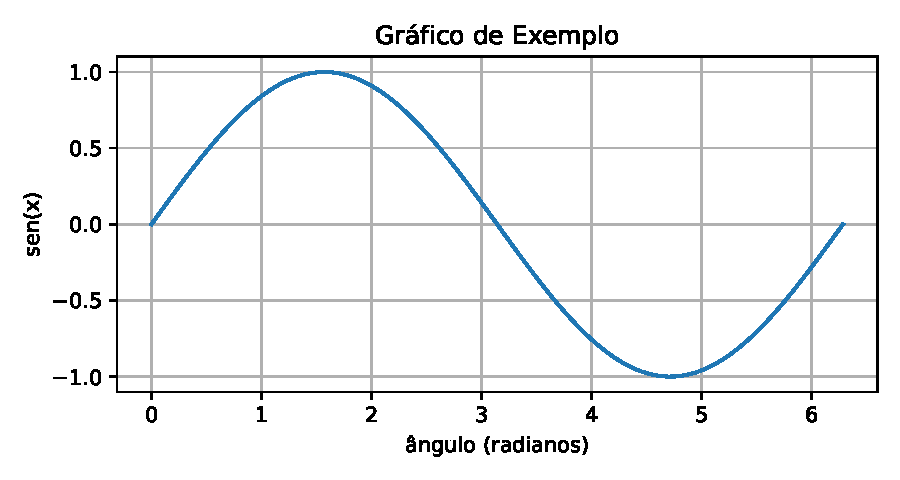
\includegraphics[width=0.8\textwidth]{figs/seno}
\end{center}
